\documentclass[pdf]{beamer}
\usepackage[slovak]{babel}
\usepackage[utf8]{inputenc}
\usepackage{hyperref}
\usepackage{breakurl} 
\usepackage{listings}

\lstdefinelanguage{JavaScript}{
  keywords={typeof, new, true, false, catch, function, return, null, catch, switch, var, if, in, while, do, else, case, break, then, yield, const, ajax},
  basicstyle=\small,
  keywordstyle=\color{blue}\bfseries,
  ndkeywords={class, export, boolean, throw, implements, import, this},
  ndkeywordstyle=\color{darkgray}\bfseries,
  identifierstyle=\color{black},
  sensitive=false,
  comment=[l]{//},
  morecomment=[s]{/*}{*/},
  commentstyle=\color{purple}\ttfamily,
  stringstyle=\color{red}\ttfamily,
  morestring=[b]',
  morestring=[b]",
  frame=lines,
  numbers=left,
  basicstyle=\scriptsize,
  numberstyle=\scriptsize,
  stepnumber=1,
  numbersep=8pt,
  showstringspaces=false,
  captionpos=b
}
\renewcommand{\lstlistingname}{Code sample}


\title[Obecné konfigurační rozhraní pro virtuální stroje \hspace{10mm} \insertframenumber/\inserttotalframenumber]{Obecné konfigurační rozhraní pro virtuální stroje}
\subtitle{Bakalárska práca}
\author{Martin Krajňák}
\date{2017}

\usetheme{Warsaw}

\begin{document}

\begin{frame}
\titlepage
\end{frame}


\begin{frame}
\frametitle{Motivácia: súčasný stav - oVirt WebAdmin}
\begin{itemize}
\item technológia GWT už nie je v aktívnom vývoji (Google)
\item súčasná implementácia je:
\begin{itemize}
\item pomalá
\item náchylná na chyby, problém so stavom dialógu
\item s pribudajúcim kódom vzniká viac chýb (callback hell)
\end{itemize}
\item virtuálny stroj 
\begin{itemize}
\item veľký počet závislostí, ktoré su vzájomne ovplyvniteľné
\item chýbajúca dokumentácia závislostí
\end{itemize}
\end{itemize}
\end{frame}


\begin{frame}
\frametitle{Ciele práce - projekt oVirt WebUI}
\begin{block}{Backend}

\begin{itemize}
\item oVirt REST API
\item ManageIQ REST API
\end{itemize}

\end{block}

\begin{block}{Redux-saga middleware}
\begin{itemize}
\item Redux-saga:
\begin{itemize}
\item asynchrónne operácie, závislosti virtuálneho stroja
\item konverzia entít na vnútornú reprezentáciu
\end{itemize}
\end{itemize}
\end{block}

\begin{block}{Frontend - ReactJS}
\begin{itemize}
\item návrh komponent s dôrazom na znovupoužiteľnosť
\item návrh hlavných komponent - dialógov
\item použitie štýlov z knižnice Patternfly
\end{itemize}
\end{block}

\end{frame}

\begin{frame}
\frametitle{Realizácia}

\begin{figure}[h]
\center{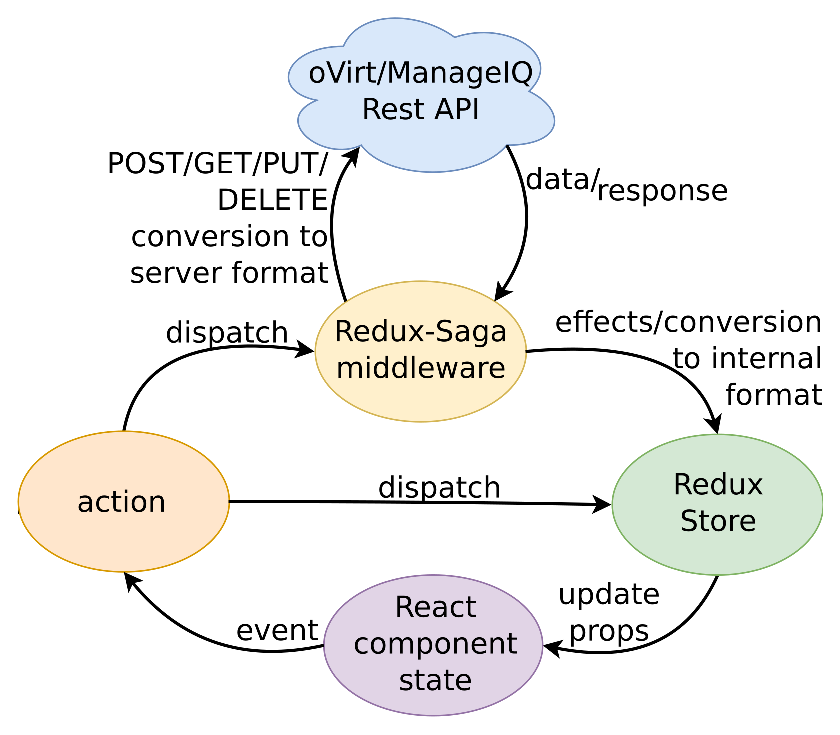
\includegraphics[scale=0.6]{application_architecture.eps}}
\label{labelledSelect}
\end{figure} 

\end{frame}

\begin{frame}
\frametitle{oVirt REST API vs ManageIQ REST  API}

\begin{block}{oVirt REST API} 
podpora takmer všetkých vlastností a akcií
\end{block}

\begin{block}{ManageIQ - problémy pri implementácii} 
\begin{itemize}
\item nefunkčná CORS implementácia:

\begin{enumerate}
\item nahlásenie problému
\item aplikovanie a testovanie navrhnutých opráv
\item problém vyriešený len čiastočne - entity najvyššej úrovne
\item dočasné riešenie - absolútne vypnutie bezpečnosti prehliadača
\end{enumerate}

\item nedostatočné/žiadne pokrytie entít
\begin{enumerate}
\item chýbajúce informácie a akcie
\item neschopnosť určenia základných vzťahov (šablona, cluster)
\end{enumerate}

\item zlé rozloženie virtuálnych strojov - spomaľovanie

\end{itemize}
\end{block}

\end{frame}

\begin{frame}
\frametitle{Realizácia}

\begin{figure}[h]
\center{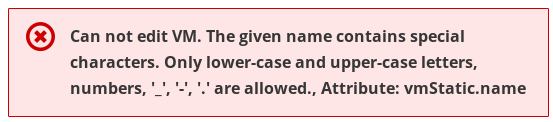
\includegraphics[width=6cm]{alert.png}}
\label{labelledSelect}
\end{figure}

\begin{figure}[h]
\center{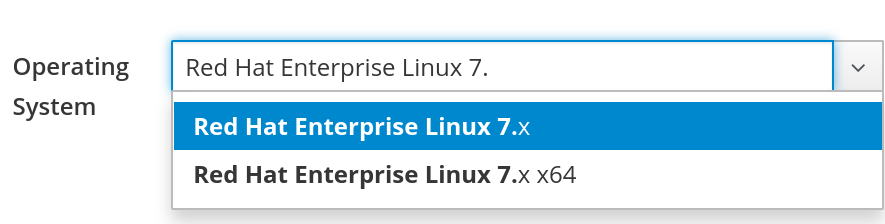
\includegraphics[width=6cm]{LabeledSelect.png}}
\label{labelledSelect}
\end{figure} 

\begin{figure}[h]
\center{
\includegraphics[width=6cm]{LabelledTextField-number.png}}
\label{labelledSelect}
\end{figure} 


\begin{figure}[h]
\center{
\includegraphics[width=2cm]{LabeledSwitch.png}}
\label{labelledSelect}
\end{figure}

\end{frame}

\begin{frame}
\frametitle{Zhodnotenie výsledkov}

\begin{itemize}
\item vypracovanie kompletného grafu závislostí virtuálneho stroja (62 položiek)
\item doimplementovanie metód oVirt API modulu
\item implementácia ManageIQ API modulu
\item riešenie závislostí entít pomocou generátorových funkcií
\item riešenie jednotného stavu dialógov - Redux
\item implementácia a testovanie alternatívneho riešenia - stav dialógov spravovaný v ReactJS
\item integrácia štýlov Patterfly knižnice a riešenie problémov spojených s~použitím jQuery
\item implementácia dialógu virtuálneho stroja
\begin{itemize}
\item umožňuje vytvorenie a úpravu virtuálnych strojov
\item menšia verzia dialógu bola úspešne zahrnutá v projekte oVirt~WebUI
\end{itemize}
\item implementácia dialógu pre úpravu šablón virtuálneho stroja
\end{itemize}

\end{frame}

\end{document}